\documentclass[11pt]{article}
\usepackage[UTF8]{ctex}
\usepackage{enumerate}
\usepackage{enumitem}
\usepackage{diagbox}
\usepackage{subfigure}
\usepackage{geometry}
\usepackage{float}
\setlist{
    leftmargin = .1\linewidth,
    % rightmargin = .1\linewidth,
    % label=\emph{\alph*}.
}

%%%%%%%%%%%%%%%%%%%%%%%%%%%%%%%%%%%%%%%%%
% Cleese Assignment
% Structure Specification File
% Version 1.0 (27/5/2018)
%
% This template originates from:
% http://www.LaTeXTemplates.com
%
% Author:
% Vel (vel@LaTeXTemplates.com)
%
% License:
% CC BY-NC-SA 3.0 (http://creativecommons.org/licenses/by-nc-sa/3.0/)
%
%%%%%%%%%%%%%%%%%%%%%%%%%%%%%%%%%%%%%%%%%

%----------------------------------------------------------------------------------------
%	PACKAGES AND OTHER DOCUMENT CONFIGURATIONS
%----------------------------------------------------------------------------------------

\usepackage{lastpage} % Required to determine the last page number for the footer

\usepackage{graphicx} % Required to insert images

\setlength\parindent{0pt} % Removes all indentation from paragraphs

\usepackage[most]{tcolorbox} % Required for boxes that split across pages

\usepackage{booktabs} % Required for better horizontal rules in tables

\usepackage{listings} % Required for insertion of code

\usepackage{etoolbox} % Required for if statements

\usepackage{amsmath}
\usepackage{amsthm}
\usepackage{amssymb}
\usepackage{indentfirst}
\usepackage{diagbox}
\usepackage{subfigure}
\usepackage{float}
\usepackage{xcolor}
\usepackage[colorlinks, linkcolor = black]{hyperref}

\usepackage{enumerate}
\usepackage{enumitem}
\setlist{
    leftmargin = .1\linewidth,
    % rightmargin = .1\linewidth,
    % label=\emph{\alph*}.
}

\setlength{\parindent}{2em}

\usepackage{siunitx}
\sisetup
{
    output-exponent-marker = \ensuremath{\mathrm{E}},
    exponent-product = {},
    retain-explicit-plus,
    retain-zero-exponent,
}
%----------------------------------------------------------------------------------------
%	MARGINS
%----------------------------------------------------------------------------------------

\usepackage{geometry} % Required for adjusting page dimensions and margins

\geometry{
    paper=a4paper, % Change to letterpaper for US letter
    top=3cm, % Top margin
    bottom=3cm, % Bottom margin
    left=2.5cm, % Left margin
    right=2.5cm, % Right margin
    headheight=14pt, % Header height
    footskip=1.4cm, % Space from the bottom margin to the baseline of the footer
    headsep=1.2cm, % Space from the top margin to the baseline of the header
    %showframe, % Uncomment to show how the type block is set on the page
}

%----------------------------------------------------------------------------------------
%	FONT
%----------------------------------------------------------------------------------------

\usepackage[utf8]{inputenc} % Required for inputting international characters
\usepackage[T1]{fontenc} % Output font encoding for international characters

% \usepackage[sfdefault,light]{roboto} % Use the Roboto font

%----------------------------------------------------------------------------------------
%	HEADERS AND FOOTERS
%----------------------------------------------------------------------------------------

\usepackage{fancyhdr} % Required for customising headers and footers

\pagestyle{fancy} % Enable custom headers and footers

\lhead{\small\assignmentClass} % Left header; output the instructor in brackets if one was set
\chead{\small\assignmentTitle} % Centre header
\rhead{\small\ifdef{\assignmentAuthorName}{\assignmentAuthorName}{\ifdef{\assignmentDate}{Due\ \assignmentDate}{}}} % Right header; output the author name if one was set, otherwise the due date if that was set

\lfoot{} % Left footer
\cfoot{\small Page\ \thepage\ of\ \pageref{LastPage}} % Centre footer
\rfoot{} % Right footer

\renewcommand\headrulewidth{0.5pt} % Thickness of the header rule

%----------------------------------------------------------------------------------------
%	MODIFY SECTION STYLES
%----------------------------------------------------------------------------------------

\usepackage{titlesec} % Required for modifying sections

%------------------------------------------------
% Section

\titleformat
{\section} % Section type being modified
[block] % Shape type, can be: hang, block, display, runin, leftmargin, rightmargin, drop, wrap, frame
{\Large\bfseries} % Format of the whole section
{\arabic{section}} % Format of the section label
{6pt} % Space between the title and label
{} % Code before the label

\titlespacing{\section}{0pt}{0.5\baselineskip}{0.5\baselineskip} % Spacing around section titles, the order is: left, before and after

%------------------------------------------------
% Subsection

\titleformat
{\subsection} % Section type being modified
[block] % Shape type, can be: hang, block, display, runin, leftmargin, rightmargin, drop, wrap, frame
{\itshape} % Format of the whole section
{(\arabic{subsection})} % Format of the section label
{4pt} % Space between the title and label
{} % Code before the label

\titlespacing{\subsection}{0pt}{0.5\baselineskip}{0.5\baselineskip} % Spacing around section titles, the order is: left, before and after

\renewcommand\thesubsection{(\arabic{subsection})}

%----------------------------------------------------------------------------------------
%	CUSTOM QUESTION COMMANDS/ENVIRONMENTS
%----------------------------------------------------------------------------------------



% Command to print an assignment section title to split an assignment into major parts
\newcommand{\assignmentSection}[1]{
    \newpage
    {
        \centering % Centre the section title
        \vspace{2\baselineskip} % Whitespace before the entire section title

        \rule{0.8\textwidth}{0.5pt} % Horizontal rule

        \vspace{0.75\baselineskip} % Whitespace before the section title
        {\LARGE \textsc{#1}} % Section title, forced to be uppercase

        \rule{0.8\textwidth}{0.5pt} % Horizontal rule

        \vspace{\baselineskip} % Whitespace after the entire section title
    }
    \setcounter{section}{0}

}

%----------------------------------------------------------------------------------------
%	TITLE PAGE
%----------------------------------------------------------------------------------------

\author{\textbf{\assignmentNo\ \assignmentAuthorName}} % Set the default title page author field
\date{} % Don't use the default title page date field

\title{
    \thispagestyle{empty} % Suppress headers and footers
    \vspace{0.2\textheight} % Whitespace before the title
    \textbf{\assignmentClass}\\[5pt]
    \texttt{\assignmentTitle}\\[-4pt]
    % \ifdef{\assignmentSubTitle}{\texttt{\assignmentSubTitle}}{}
    \ifdef{\assignmentDate}{\assignmentDate}{} % If a due date is supplied, output it
    \ifdef{\assignmentClassInstructor}{{\large \textit{\assignmentClassInstructor}}}{} % If an instructor is supplied, output it
    \vspace{0.32\textheight} % Whitespace before the author name
}
 % Include the file specifying the document structure and custom commands


\newcommand{\assignmentQuestionName}{Question} % The word to be used as a prefix to question numbers; example alternatives: Problem, Exercise
\newcommand{\assignmentClass}{计算方法B} % Course/class
\newcommand{\assignmentTitle}{Programming Assignment\ \#2} % Assignment title or name
\newcommand{\assignmentDate}{2020.4.6} % date
\newcommand{\assignmentNo}{PB17000297}
\newcommand{\assignmentAuthorName}{罗晏宸} % Student name

\begin{document}

\maketitle % Print the title page

\thispagestyle{empty} % Suppress headers and footers on the title page

\newpage

\assignmentSection{Question 1}
\section{问题描述}
对函数$\displaystyle f(x) = \frac{1}{2 + 2x + x^2},\ x \in [-5, 5]$,构造其$N$次 Lagrange 插值函数,取
\begin{equation*}
    \max_{-5 \leqslant x \leqslant 5}{\left \Arrowvert f(x) - p(x)\right \Arrowvert } \approx \max_i{\left\arrowvert f(y_i) - p(y_i)\right\arrowvert},\ y_i = \dfrac{i}{50} - 5,\ i = 0,\, \cdots,\, 500
\end{equation*}
为近似误差。其中,插值结点(设有$N + 1$个)取为:
\begin{enumerate}[label = (\arabic*)]
    \item $x_i = -5 + \dfrac{10}{N}i,\, i = 0,\,1,\,\cdots,\,N$
    \item $x_i = -5\cos{\left(\dfrac{2i + 1}{2N + 2}\pi\right)},\, i = 0,\,1,\,\cdots,\,N$
\end{enumerate}
对$N = 4,\ 8,\ 16$比较以上两组结点的插值结果。

\section{计算结果}
由C++计算得到结果按格式输出如图\ref{Output}所示,
\begin{figure}[H]
    \centering
    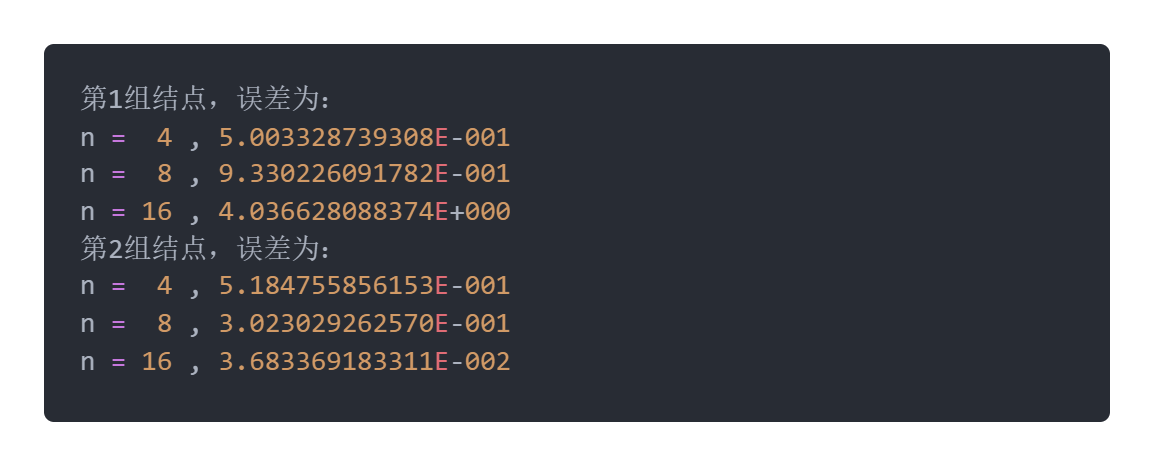
\includegraphics[scale = 0.35]{Output.png}
    \caption{C++程序的运行结果}
    \label{Output}
\end{figure}
其中数据可列如表\ref{table}。
\begin{table}[h]
    \centering
    \begin{tabular}{|c|c|c|}
        \hline
        \diagbox{结点数}{近似误差}{插值结点} & 均匀等距选取                 & Chebyshev多项式零点          \\
        \hline $N = 4$                       & $5.003328739308\text{E}-001$ & $5.184755856153\text{E}-001$ \\
        \hline $N = 8$                       & $9.330226091782\text{E}-001$ & $3.023029262570\text{E}-001$ \\
        \hline $N = 16$                      & $4.036628088374\text{E}+000$ & $3.683369183311\text{E}-002$ \\
        \hline
    \end{tabular}
    \caption{$N = 4,\ 8,\ 16$时两组插值结点的近似误差}
    \label{table}
\end{table}
使用Mathematica统计数据并绘图,列如图\ref{curves}。
\begin{figure}[H]
    \centering
    \subfigure[$N = 4$时均匀插值结点构造的插值函数图像]{
        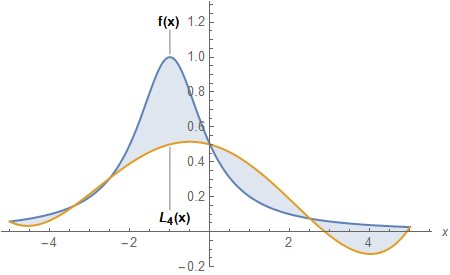
\includegraphics[scale = 0.45]{Linear_N=4.png}
    }
    \quad
    \subfigure[$N = 4$时Chebyshev插值结点构造的插值函数图像]{
        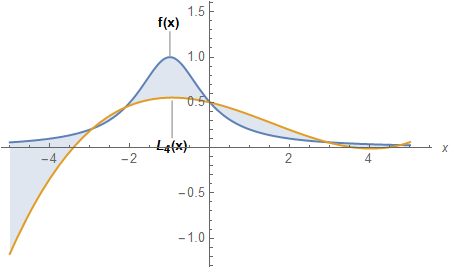
\includegraphics[scale = 0.45]{Chebyshev_N=4.png}
    }

    \subfigure[$N = 8$时均匀插值结点构造的插值函数图像]{
        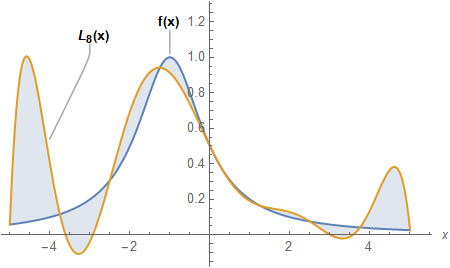
\includegraphics[scale = 0.45]{Linear_N=8.png}
    }
    \quad
    \subfigure[$N = 8$时Chebyshev插值结点构造的插值函数图像]{
        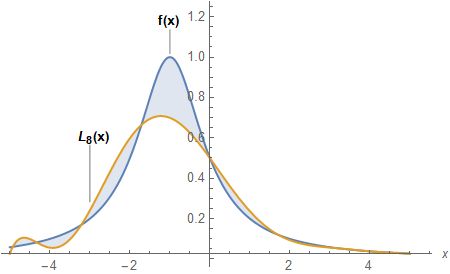
\includegraphics[scale = 0.45]{Chebyshev_N=8.png}
    }

    \subfigure[$N = 16$时均匀插值结点构造的插值函数图像]{
        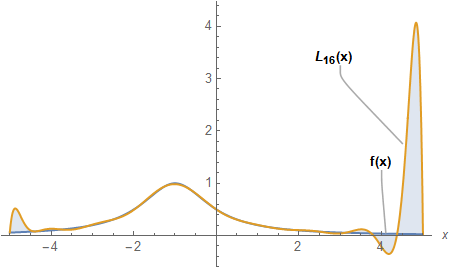
\includegraphics[scale = 0.45]{Linear_N=16.png}
    }
    \quad
    \subfigure[$N = 16$时Chebyshev插值结点构造的插值函数图像]{
        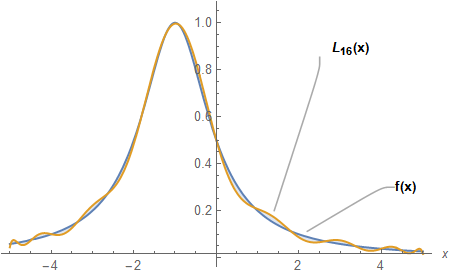
\includegraphics[scale = 0.45]{Chebyshev_N=16.png}
    }
    \caption{$N = 4,\ 8,\ 16$时两组插值函数与$f(x)$的图像}
    \label{curves}
\end{figure}
\section{结果分析}
从近似误差的结果来看,随着结点数(插值多项式次数)增加,均匀选取结点构造的插值多项式函数反而出现了误差增加的现象,同时使用相同数量的Chebyshev多项式零点构造的插值多项式误差相比均匀选取较小,并且误差随结点数增加而减少。

从$N$取不同值时两组插值结点构造的函数图像来看,整体上,在区间$[-4, 4]$上,插值结点越多,两组插值函数的拟合效果都越好。对于均匀选取的插值结点构造的插值函数,当$N = 16$时,区间$[-4, 4]$上函数图像偏差很小,可以较好地逼近$f(x)$,但在边界$x = -5$或$x = 5$附近,插值函数和$f(x)$的图像偏差很大,插值多项式函数出现了剧烈的振荡。对于使用Chebyshev多项式零点构造的插值函数,在包括边界的整个区间上,图像偏差都很小。

以上均匀选取插值结点构造的多项式函数产生的现象说明了高次多项式的插值效果不一定优于低次多项式,同时等距插值不能保证较好的插值效果,是典型的Runge现象。

Lagrange 插值多项式的截断误差由下式给出:
\begin{equation*}
    f(x) - L_n(x) = \frac{f^{(n + 1)}(\xi)}{(n + 1)!}(x - x_0)(x - x_1)\cdots(x - x_n), \quad \xi \in [a, b]
\end{equation*}
其中$[a, b]$在这里是$[-5, 5]$,使用Chebyshev多项式零点构造插值函数,即当$$x_i = -5\cos{\left(\dfrac{2i + 1}{2N + 2}\pi\right)},\, i = 0,\,1,\,\cdots,\,N$$时有:
\begin{align*}
    \max_{-5 \leqslant x \leqslant 5}{\left \Arrowvert f(x) - p(x)\right \Arrowvert} & = \max_{-5 \leqslant x \leqslant 5}{\left \arrowvert\frac{f^{(N + 1)}(\xi)}{(N + 1)!}(x - x_0)(x - x_1)\cdots(x - x_N)\right \arrowvert}                       \\
                                                                                     & = \left \arrowvert \frac{f^{(N + 1)}(\xi)}{(N + 1)!}\right \arrowvert \max_{-5 \leqslant x \leqslant 5}{\arrowvert(x - x_0)(x - x_1)\cdots(x - x_N)\arrowvert} \\
                                                                                     & \leqslant \left \arrowvert \frac{f^{(N + 1)}(\xi)}{(N + 1)!} \right \arrowvert \frac{5^{N + 1}}{2^N}                                                           \\
                                                                                     & = \frac{5^{N + 1}}{2^N(N + 1)!} \left \arrowvert f^{(N + 1)}(\xi) \right \arrowvert, \qquad \xi \in [-5, 5]                                                    \\
                                                                                     & \leqslant \frac{5^{N + 1}}{2^N(N + 1)!} \max_{\xi \in [-5, 5]}{\left \arrowvert f^{(N + 1)}(\xi) \right \arrowvert}
\end{align*}
因此能够限制插值函数误差的上界。

由Mathematica计算得到当$N = 4,\ 8,\ 16$时,误差的数值上界可列为表\ref{table2}。
\begin{table}[h]
    \centering
    \begin{tabular}{|c|c|c|}
        \hline
        插值结点数 & $\displaystyle \frac{5^{N + 1}}{2^N(N + 1)!}$ & $\displaystyle \frac{5^{N + 1}}{2^N(N + 1)!} \max_{\xi \in [-5, 5]}{\left \arrowvert f^{(N + 1)}(\xi) \right \arrowvert} $ \\ \hline
        $N = 4$    & $1.627604166667\text{E}+000$                  & $1.635074592041\text{E}+002$                                                                                               \\ \hline
        $N = 8$    & $2.102456605834\text{E}-002$                  & $6.817348655088\text{E}+003$                                                                                               \\ \hline
        $N = 16$   & $3.272967010673\text{E}-008$                  & $1.090883874366\text{E}+007$                                                                                               \\ \hline
    \end{tabular}
    \caption{$N = 4,\ 8,\ 16$时使用Chebyshev多项式零点构造插值函数的误差上界}
    \label{table2}
\end{table}
可以看到,此前使用Chebyshev多项式零点构造插值函数产生的误差明显小于表\ref{table2}第三列给出的上界,事实上这个上界很大,同时注意到第二列指出的系数是很小的,
\begin{figure}[H]
    \centering
    \subfigure[$f^{(5)}(x)$的函数图像]{
        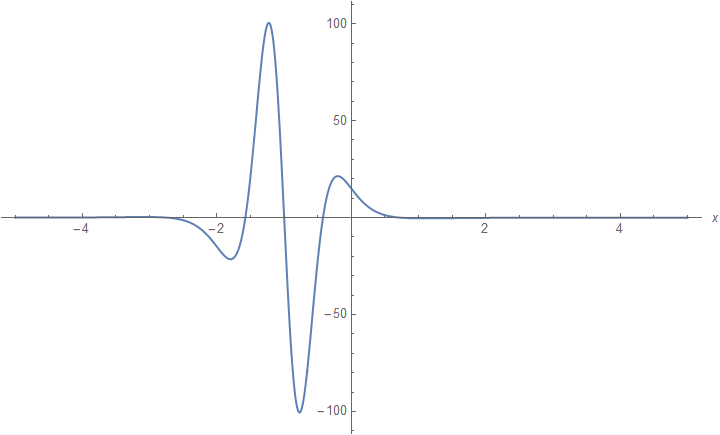
\includegraphics[scale = 0.25]{5th_Derivative.png}
    }
    \quad
    \subfigure[$f^{(9)}(x)$的函数图像]{
        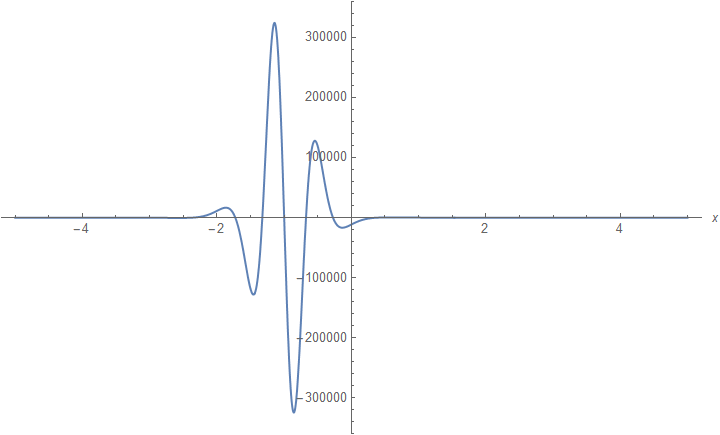
\includegraphics[scale = 0.25]{9th_Derivative.png}
    }

    \subfigure[$f^{(17)}(x)$的函数图像]{
        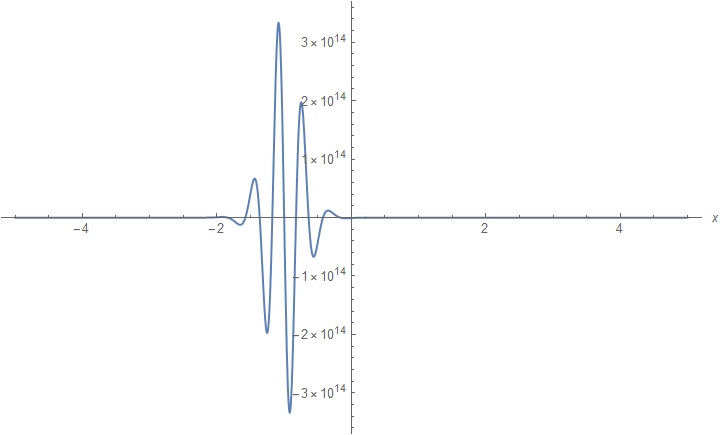
\includegraphics[scale = 0.25]{17th_Derivative.png}
    }
    \caption{$f(x)$的各阶导函数图像}
    \label{Derivative_curves}
\end{figure}
结合图\ref{Derivative_curves}可知,以此法估计的上界较大以至于失去参考价值,主要是因为$f(x)$的各阶导函数在区间$[-2, 0]$上有较大的振荡,其在$[-5, -2) \cap (0, 5]$上的函数值是较小的。

\section{算法分析}
在本实验的C++程序实现中,采用 Lagrange 基函数构造插值多项式
\begin{equation*}
    L_n(x) = \sum_{i = 0}^n{\prod_{0 \leqslant j \leqslant n, j \ne i}{\frac{x - x_j}{x_i - x_j}}f(x_i)}
\end{equation*}
随着插值多项式次数的增加,其中基函数$l_i(x) = \displaystyle \prod_{0 \leqslant j \leqslant n, j \ne i}{\frac{x - x_j}{x_i - x_j}}$在程序中的浮点数连乘计算会产生舍入误差的放大,这是高次插值多项式的另一个缺陷。

\section{实验结论}
本次实验是体现 Runge 现象的另一个例子,展示了插值多项式在插值区间内发生剧烈振荡的现象,指出了高次插值多项式的缺陷:插值效果并不一定随多项式次数增加而优化,等距的选取插值结点也往往不能保证插值效果。

使用Chebyshev多项式零点构造插值函数能够有效遏制 Runge 现象,避免插值函数的剧烈振荡,其理论基础是限制了插值多项式截断误差的上界,使其取得最小值。
\end{document}
